\documentclass[11pt, a4paper, oneside, openright, medskipamount]{report}

\usepackage{float}
\usepackage{url}
\usepackage{enumitem}
\usepackage{pifont}
\usepackage[utf8]{inputenc}
\usepackage[english]{babel}

\setlength{\parindent}{0em}
\setlength{\parskip}{1em}
\renewcommand{\baselinestretch}{1.1}

\newfloat{fig}{thp}{lof}[chapter]
\floatname{fig}{Figure}

\title{%
Tutorial Builder \\
\large Final Report}

\author{Zoltan Debre}

% Victoria University ECS
\usepackage[image,ecs,mcompsci]{vuwproject}

\supervisor{Dr Stuart Marshall}

\date{16th October 2016}

\begin{document}

\frontmatter

\begin{abstract}

Presenting a computer programming problem or solution to learners with a high-quality video is time-consuming and it is not easy to update.

Technical content producers are struggling to find an efficient and interactive way to show their work.

This research introduces a experimental prototype that can be a conceptual tool for creating an interactive tutorial.

Furthermore, this prototype shows programming code snippets in web based code editor so the content creator can build a playable step by step "movie" with it.

Project source code: \url{http://github.com/zoltan-nz/tutorial-builder}

\end{abstract}


%%%%%%%%%%%%%%%%%%%%%%%%%%%%%%%%%%%%%%%%%%%%%%%%%%%%%%%

\maketitle

\tableofcontents

%%%%%%%%%%%%%%%%%%%%%%%%%%%%%%%%%%%%%%%%%%%%%%%%%%%%%%%

\mainmatter

%%%%%%%%%%%%%%%%%%%%%%%%%%%%%%%%%%%%%%%%%%%%%%%%%%%%%%%

\chapter{Introduction}

This project is about building an online publishing prototype, using code editors, and step by step instructions to present programming challenges and solutions for a computer science related problem.

The prototype has two parts, an administration area, where the content creator can build a tutorial, and a player tool, where the recorded steps will be presented.

The primary target user is the creator, who composes new tutorials. The creator can be a teacher, or an open source project owner, who would like to introduce their tool or code.

The secondary user is the consumer, who wants to learn or know more about a problem or a coding solution.

\section{Motivation}

We all have the unstoppable desire to learn. We are keen to know more about the world around us, about our hobby and our profession. In software development, in computer science, the knowledge is essential, it is the key to succeeding. Reading, studying, sharing. An infinite loop of collecting and adapting new practices.

In information technology, especially in programming languages, writing blog posts, creating static, step by step tutorials are a popular way to share or learn something new. Producing and sharing the content is easier nowadays, but still requires more effort from the creator, when they want to deliver an easy to understand high-quality tutorials.

Creating interactive tutorials are appealing, but the production cost is much higher. Recording a video tutorial or especially updating it is time-consuming, and it involves more effort from the creator.

I think an ideal solution would be a healthy mix of static and dynamic content, where learners can read instructions meanwhile they can watch the steps in a code editor, in a more realistic environment.

\section{The problem}

When a developer, teacher or hobbyist would like to present a computer programming problem or solution, most of the times they record a video, and publish it on YouTube. However recording and editing a high-quality video is time-consuming and less flexible. It is also hard to update.

Other problem with showing tutorials with a simple video, that the audience cannot give it a try, they have to configure their computer and environment to play with the presented solution.

Most of the cases we would like to show instructions and code snippets, mainly text-based contents. It is preferred to show code snippets in a more realistic environment, such as in a code editor. Therefore using the online code editor with a pre-scripted way to play the presentation, where the user can navigate back and forth and can modify or play with the code is more interactive. It involves everyone and helps to understand a problem clearly.

Additionally, it is much easier to maintain, upgrade or fix for the content creator.

Furthermore, the user is able to experience it and can see the result, so the new information can be put into practice immediately.

\section{Personas and their goals}

\subsection{Primary persona}

Content creator, open source project maintainer, teacher.

Their motivation is to present a technical problem and its solution in a clear, easy-to-understand way. The best option is to show a demo, what happens when we insert the suggested code, how easy it is to use. Most of the times a presentation involves more steps. For example, we would like to show a starting state, maybe a few lines of code which we are able to simplify, so in this case, the first step is to show the problem, and after we show how we solve it step by step.

\subsection{Secondary persona}

The consumer, who watch the presentation, who reads the tutorial and who wants to learn more about the actual problem.

They would like to play, stop, and control the presentation. Control the flow, going forward or stepping back.

They would like to try the solution, for example how the final state changes when they modify the code.

\subsection{Target groups}

I develop a prototype web app, where the content producer can create a simple step by step tutorial, and the content consumer can "watch" this tutorial and can interact with it.

There are two different users:
\begin{itemize}[noitemsep]
\item content producer, for example a software developer or teacher
\item content consumer, for instance a student or another software developer who would like to learn a new tool
\end{itemize}

The content creator is a software developer with a deep technical knowledge, however they prefer if a tool is user friendly, and it can support their goal. In this case, they want to present or teach a certain technique or introduce a software library they wrote. It is important to them that they can deliver an introduction or a tutorial quickly, and they do not have to invest too much time to learn a new tool to create additional content. These tutorials are usually present a smaller problem with a few steps, and a content consumer can learn it in 3-5 minutes.

The content consumer would like to understand the tool as fast as they can, they want to try, and they would like to adopt this new knowledge in their work as soon as possible.

\chapter{Related Work}

During the development and research work, I found a few related interesting projects. These are similar or I can use them partly.

\section{CodeMirror Movie}

I found this project when I checked the most popular web-based code editor tool, CodeMirror website. The creator of the CodeMirror wanted to present their tool with a realistic way, so CodeMirror Movie was born. \cite{cm-movie}

A content creator, a tutorial builder can use CodeMirror Movie to script a step by step tutorial. There is a special scripting language which can help to build a "movie" which presents a code editing process. The content creator, our primary persona can add comments also to each step.

The content consumer, our secondary persona, who would like to learn or practice, they can watch, stop and restart this "movie". They can follow the editing process and see the comments. At the end of the tutorial, the content consumer can click in the code editor, and they are able to edit.

This solution highly coupled with CodeMirror, it is similar to an add-on, so it is possible to attach any CodeMirror implementation. (More about CodeMirror in Section \ref{comparison})

Adding CodeMirror Movie to our project is straightforward because the open source repository provides a CSS and a JS file, so they can be added to any page.

This tool mainly targets web-developers, so with the help of this tool they can add code and scripts to their websites.

Editing "the movie" script is manual. There is a simple syntax which control the presentation steps and this script should be added to the textarea which will be in the code editor.

We clearly see that it is a very effective way to build a presentation, however it requires real development skills.

Viewing this tool from our personas perspective, we can clearly state, the content creator does not get an easy to use solution. CodeMirror Movie does not have any graphical user interface for creating content, it can be managed by scripting. Easy to use graphical interface is an important requirement.

Our secondary persona, the content consumer can play and stop the tutorial, can choose individual steps and can use the code editor for experimenting with the example. From their perspective, the CodeMirror Movie is almost an ideal tool.

\noindent Pros:
\begin{itemize}[noitemsep]
\item simple, lightweight implementation
\item easy to add your project if you use CodeMirror and you are a developer
\item simple script language to manage the presentation
\item user can use the code editor to try the presented solution
\end{itemize}
Cons:
\begin{itemize}[noitemsep]
\item mainly for developers only
\item highly coupled with CodeMirror
\end{itemize}

\section{Comparison of online code editors} \label{comparison}

There are three popular web based code editors: CodeMirror, Ace Editor and Monaco.

CodeMirror and Ace Editor are commonly used on websites and different projects. Monaco is a new solution from Microsoft and it is extracted from their popular Microsoft Visual Studio Code developer tool.

There is not significant differences between them. All has the most important code editor features, like supporting more than 100 languages, autocompletion, syntax highlighting, controlling with shortcuts.

I will use CodeMirror in my prototype, because it has already Ember.js support. Thanks for the ivy-codemirror Ember addon, it can be added to any Ember.js project with the installation of the addon. More about the implementation in Section \ref{codemirror}.

\noindent CodeMirror
\begin{itemize}[noitemsep]
\item Github link: \url{https://github.com/codemirror/CodeMirror}
\item Website: \url{http://codemirror.net/}
\item Popularity (GitHub Star): 9396
\item Ember.js Addon: \url{https://www.emberobserver.com/addons/ivy-codemirror}
\end{itemize}

\noindent Ace Editor
\begin{itemize}[noitemsep]
\item Github link: \url{https://github.com/ajaxorg/ace}
\item Website: \url{https://ace.c9.io}
\item Popularity (GitHub Star): 12950
\item Ember.js Addon: none
\end{itemize}

\noindent Monaco
\begin{itemize}[noitemsep]
\item Github link: \url{https://github.com/Microsoft/monaco-editor}
\item Website: \url{https://microsoft.github.io/monaco-editor/}
\item Popularity (GitHub Star): 2322
\item Ember.js Addon: none
\end{itemize}

A good code editor is an important part of any tutorial builder. The content creator persona prefers a code editor which helps in editing and autocompleting, also it is able to save the history of the editing process and supports undo and redo features.

A content consumer persona can process the content faster, if the code editor supports highlighting, the code is strictly structured and formatted with proper indentation.

\section{Reviewing code sharing websites}

We can use code editor and sharing platforms also when we want to demo a small feature or describe a problem. These websites are combinations of code editors and an iframe where we can see the preview of the code snippets.

One of the common features is splitting the screen and providing different windows for editing html, css and javascript separately.

User can save the edited content also. Most of them can be embed in a blog post or in other website.

\noindent Most important findings:
\begin{itemize}[noitemsep]
\item All use Code Mirror as code editor
\item All of them separate the css, html and javascript editing in different screens, but they merge into one file, and preview of this merged html file is possible in an iframe.
\item Saving the different type of code (css, javascript, html) separately.
\end{itemize}

Our target group, content and tutorial creators use code sharing websites for demonstrating solutions. The main problem with code sharing websites that they show a static state, mainly the final version of a tutorial. As a result the content consumer can not see the interim steps.

Comparison of the code sharing websites is in Figure \ref{fig:code-sharing-website-review}

\begin{figure}[ht]
\centering
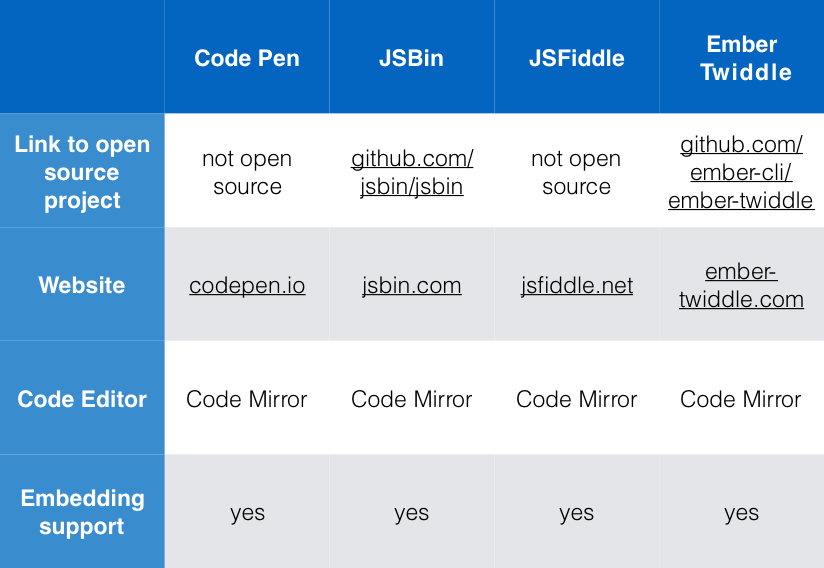
\includegraphics[width=1\textwidth]{assets/code-sharing-website-review}
\caption{Code sharing website review}
\label{fig:code-sharing-website-review}
\end{figure}

\chapter{Design}

\section{Requirements}

We have seen in our previous chapter, there are tools that provide limited solution for tutorial builders and tutorial consumers. However, a combination of these tools would support more our primary and secondary personas.

Our goal is to design a system, which can solve the problems explained above. Content creators can easily create and maintain their introduction, add and remove steps in a graphical user interface while providing enough examples to other developers or learners, and also keeping the different types of content separately in the editor tool. (R1-R6, R12, R13)

A learner want to navigate easily between different content, watch the examples, see the interim steps and try them in a code editor. (R7-R11, R14)

A fully functional tutorial service could have the following requirement list. We can separate them in three different groups. One group focuses on requirements for the tutorial creator/admin/teacher, and an other group for the consumer/students and a separate group of requirements for user interface considerations.

\noindent Requirements from the teacher perspective:
\begin{itemize}[noitemsep]
\item Teacher can navigate to Admin page. (R1)
\item Teacher can create a new tutorial. (R2)
\item Teacher can add steps to the tutorial. (R3)
\item A step can have different types of content. (R4)
\begin{itemize}[noitemsep]
\item Instruction type is a text content.
\item Html type, which adds content to the html editor box.
\item Css type, which adds content to the css editor box.
\item JavaScript type, which adds content to the javascript editor box.
\end{itemize}
\item Teacher can modify the content of a step later. (R5)
\item Steps are always in sync, so the next step always inherits the previous step state. (R6)
\end{itemize}

\noindent Requirements from the student perspective:
\begin{itemize}[noitemsep]
\item Student can see a list of tutorials. (R7)
\item Student can click on a tutorial and can see the steps. (R8)
\item Steps are presented in order. (R9)
\item Student can "play" and "watch" the steps. (R10)
\item Student can "pause" and step "backward". (R11)
\end{itemize}

\noindent User interface requirements (R12):
\begin{itemize}[noitemsep]
\item The tutorial screen has three area:
\item Instruction area.
\item Code editor area (for HTML, CSS and JavaScript).
\item Website preview area.
\end{itemize}

\noindent The main website has two main section:
\begin{itemize}[noitemsep]
\item Admin page where Teacher can edit tutorials. (R13 - The Builder)
\item Tutorials page where Students can select and watch tutorials and can edit the code examples. (R14 - The Player)
\end{itemize}

\section{Database design considerations} \label{database-design}

One of the core element of an application is the database and model layer. Determining data entities are an important step of the planning process and it helps us in the implementation process.

In a fully featured implementation our database structure would be more complex and would cover extended use cases. Firstly, I list a wider model structure, after I will focus on models what I implemented in the prototype.

Our main problem domain is tutorials, one of the most important models is the entity where we store the different tutorials. So a "tutorial" model would have at least a "name" field. The tutorial model has many "lesson". Each lesson has a "title", a field where we can store the position, the "sort" value, and it has many "steps" also. So the smallest level of this model structure is the "step" model. Step fields: name, type, code, and sort.

Simply: Tutorial -\textgreater Lesson -\textgreater Step

More about the final implementation in Section \ref{database-implementation}.

\section{Managing history changes} \label{history}

In a step by step tutorial builder, one of the core functionalities is adding steps to a tutorial. It is important also that we should be able to edit, modify, delete, reorganize these steps.

A programming tutorial’s main content is code. Code has lines. Usually in the first step we add a few lines, so there will be two-three lines of code in the code editor. In the next steps we add more and more. We extend lines, remove lines. Each step is based on the previous state, the code in the code editor incrementally changes.

Let's say we have 4-5 steps and we would like to remove the code what we saved in the Step 3. After these changes, Step 2 should be the start state of the Step 4, so we should manually adjust Step 4 starting state to be the same as the end state of the Step 2. We can show the difference between the final state of the Step 2 and the actual start state of the Step 4 with highlighting, and we can ask the user to adjust the code. This process looks simple when we talk about a few lines of code. However, when we build a bigger tutorial, this adjustment process could be a nightmare.

I was thinking about this problem a lot, and I tried to use the following simplification to solve this problem.

One of the ideas is creating a snapshot at the beginning of a step and at the final state of a step.

In the following abstraction, H1, H2... are history elements, they represent actions. S1, S2... are steps. L1, L2... are lines of code.

\begin{itemize}[noitemsep]
\item H1. Snapshot N1, "Empty state"
\item H2. Create Step S1, add Line L1
\item H3. Snapshot N2 = H1 + H2.
\item H4. Create Step S2, add Line L2
\item H5. Snapshot N3 = H3 + H4
\item H6. Modify Step S1, add new Line after L1
\item H7. Update Snapshot N2 = H1 + H2 + H6
\item H8. Update Snapshot N3 = H7 + H3
\end{itemize}

In this concept a snapshot is like a pointer, which collects together the connected history elements.

However, this concept can work only if all the changes made in the code editor saved as relative changes. For example, if I have something in the Line 1 and we add something else in the Line 2, I save the changes as "add a line after the last line of the previous step", so if we delete the Step 1, the relative instruction still can work.

Unfortunately, managing relative history is not possible with Code Mirror at the moment. My plan is to extend the tool with this feature in a following project.

I was thinking about another theory. We use git. Git main feature is tracking changes. It keeps the differences between two commits, so we can see what happens between two commits. These changes stored as relative changes also. However, one of the strict restrictions in git, which is an important feature, we cannot easily modify the history of commits. When we would like to override the history, we actually has to make a copy from the git repository.

In this case, the problem is the same again as I described above. How can we match the previous step final state with the next step start state. When we use git and we try to commit a change which collide with other change git raises a "conflict". The user has to manually resolve this problem. So we are on the same path again with this theory also: manual resolving.

The answer for this problem that we cannot avoid from manual resolving, however we can make it more comfortable with a user friendly implementation.

\section{User experience}

\subsection{Step builder wireframe}

The Step Builder is one of the core elements of our application. Our main content creator persona will use this form to add a new content, a new step to the tutorial.

The Figure \ref{fig:step-builder-wireframe} shows the important fragments of the interface. A vertical box can show the list of steps, a form can manage the content of a step. A preview window is also important to see the actual state of the tutorial. An advance feature is to separate content or customize the form based on the content type (css, html, JavaScript).

\begin{figure}[ht]
\centering
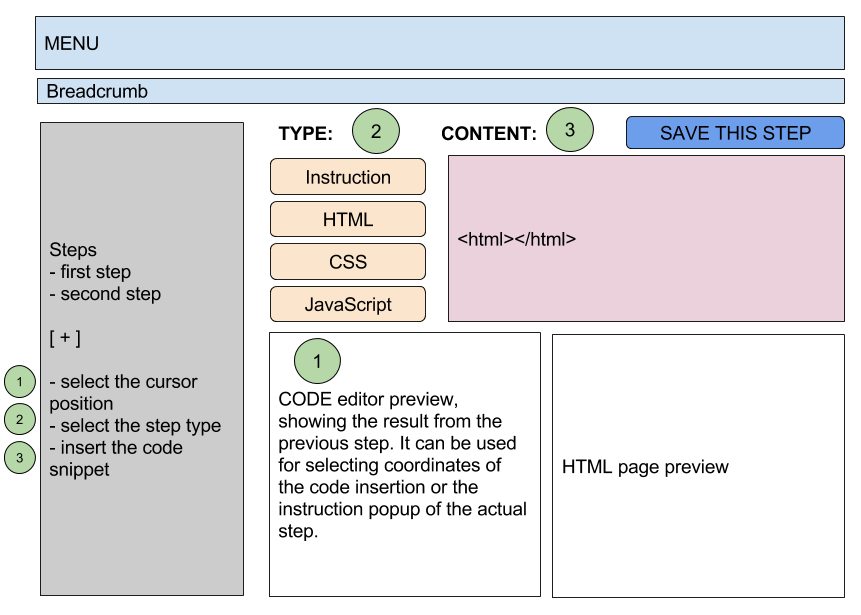
\includegraphics[width=1\textwidth]{assets/step-builder-wireframe.png}
\caption{Step Builder wireframe}
\label{fig:step-builder-wireframe}
\end{figure}

\subsection{Breadcrumbs}

One of the most important rules in UX, that the user should not be confused. When they use a website and navigate in different area, they have to know where they are. Usually below the navigation bar, there is a section, where we show the actual position of the user inside the site architecture. It is called breadcrumbs. More about the implementation in Section \ref{breadcrumbs-implementation}.

\chapter{Implementation}

\section{The story of 12 factor apps}

The Twelve-Factor App is the name of a methodology, which collects together twelve important concepts and rules what we should follow when we build a modern software-as-a-service or web application. We can find this collection on this website: \url{http://12factor.net}

I think, it is important to follow this methodology in our application also. Instead of repeating all of the 12 rules, I describe how I use a certain rule in my implementation.

1. Codebase. As it already mentioned above, our app uses one codebase, uses git and is hosted on Github and the codebase is the same across all deploys.

2. Dependencies. External dependencies of our app managed by a package manager, in our case "npm", the node package manager and "bower", for third party assets, like Ember.js or Bootstrap.

3. Config. The configuration sits separately in "config/environment.js" file, and it can be different on development mode or on production mode.

4. Backing services. The Tutorial Builder backend system is attached via an adapter to the third party database, Firebase which accessible via a direct URL. The backend works as a service.

5. Build, release, run. We can build our Ember application with a terminal command "ember build --prod", the production version of the code deployed by an other terminal command "surge".

6. Processes. This rule is relevant also in our case, because our app is a static, single page application, so it is a stateless and "share-nothing" solution.

7. Port binding. This rule would be relevant only if we would use our own server. The backend service and the static single-page application would run from this server using a web server. In this case the backend server, which is a Ruby on Rails application, would run on a different port behind the web server. For example on "http://localhost:3000/" address. However the backend service would be open to public on the same domain name as the whole application. For instance, if our Ember.js single-page application runs on "http://tutorial-builder.com/", the Ruby on Rails backend API would be available on "http://tutorial-builder.com/api".

8. Concurrency. Our single page application is stateless, basically a static website. In terms of high traffic, it is easy to clone and launch on other server. Luckily, modern static website hosting services automatically clone it on content delivery network which means, it can scale.

9. Disposability. We don't have to turn off our web application when we would like to update. We can just deploy and overwrite the previous version in a second.

10. Dev/prod parity. As a twelve-factor developer, it is important for me, that I should be able to deploy continuously. It means, I can manage the code base, update or fix it, test on the developer machine, test with the production database, build the production version and deploy immediately. With my development environment and with tools of my choice, this principle is adopted also.

11. Logs. This feature can be adopted in our environment, but it is not active in our experimental project.

12. Admin processes. Our database administration focuses only for maintaining, deleting the Firebase database, it can be done on Firebase website as a single process.

\section{The technology of choice}

One of the most popular programming languages in web development is JavaScript. The usage of this frontend focused technology is growing quickly.  It is the 7th on Tiobe Index, which is a good indicator of programming languages popularity. \cite{tiobe}

Learning and teaching JavaScript, HTML and CSS is important. My tool focuses on this three main building blocks of the web.

Building a frontend heavy application, with a dynamic, user-friendly interface is more common nowadays. In the last few years JavaScript based frontend frameworks became mature, production ready tools. Server side technologies, like database management and time and resource heavy processes are separated from the user focused, design driven view layer, which is developed with usage of frontend frameworks.

The most popular tools are Angular.js, React.js and Ember.js. In my project I use Ember.js. It is an "opinionated" framework. Opinionated, convention over configuration driven framework means that developers should follow specific conventions, instead of using the tool freely. A more strict environment helps to adopt best practices and speeds up the development process.

Certainly, we still have to store data and information, so we cannot live without backend and server technology. Luckily there are already cloud-based tools for managing databases. I use Firebase \cite{firebase}, which is a service provided by Google. Firebase is a cloud-based database, document-store solution and easy to integrate with Ember.js.

Additionally, I started building a traditional backend server application also to support development and experimenting with a real server side and a cloud-based solutions parallel. My preferred technology on backend side is Ruby on Rails, a popular, also opinionated and convention over configuration driven backend framework. However, I added only one model to this backend, because finally I just focused on the Firebase implementation.

Following the most modern standard of web applications, I separate the user faced frontend development and the data store, backend development.

The user face frontend application uses Ember.js frontend framework. Ember.js development requires Node.js on the development machine to run the development environment. This development environment helps to run and modify frontend code quickly, and it generates the final, deployable production code also. The production version of the application is only a static website. It means, there is one index.html, two JavaScript files and two CSS files.

\section{Source control management}

I have been using GitHub for managing source code and tracking code changes. Link to repository: \url{https://github.com/zoltan-nz/tutorial-builder}

\section{Static website hosting}

I have been using surge.sh \cite{surge} for static website hosting, so the actual state of the prototype is updated there regularly. Link to the live version: \url{http://tutorial-builder.surge.sh}

\section{Frontend features}

The look and feel of the application follows the standard Bootstrap style. Bootstrap is added to the project. I use "sass" version of the Bootstrap, so I can customize it with the modification of the "sass" variables. "Sass" is a modern CSS development environment that helps to modify the CSS programmatically.

The home page of the application is only a placeholder. I added a navigation bar with the following links: Home, Builder, Player, Sandboxes, and Dashboard. (Requirements R1, R2, R3, R7, R8, R13, R14.)

I implemented a breadcrumb bar also which helps in navigation.

I created a Sandbox area, where I experimented with the CodeMirror code editor. An iFrame is also added to this page which shows the preview. This Sandbox page contains the editor. When the source code is updated, the preview page automatically renders the generated website. This feature uses Ember.js default two-way bindings capability.

\section{Data down actions up}

In software architecture and computer science it is always a challenge how to write clean code \cite{clean-code}, which is always readable and easy to maintain. I built my project mainly in JavaScript, and it is known that JavaScript is not a strict language, no strict types as in Java, it does not force structured object oriented patterns. However, JavaScript has been changed a lot in the last few years, thanks to the new version. The new JavaScript standard is called ES2015 or ES6 \cite{es6}.

JavaScript with ES6 syntax and with a heavily object oriented JavaScript framework, like Ember.js, can force you to write an easy to understand, easy to maintain system. Ember.js is a Model-View-Controller type framework, and it helps to separate concerns and makes your code more SOLID \cite{solid}.

With modern JavaScript frameworks we mainly build frontend, user faced applications, so the view layer of our product is a webpage or a web component. These pages or components are a mix of static and dynamic contents. Static content is built in the presentation template, however the dynamic content is usually provided by a backend service from a database.

Modern JavaScript frameworks are adopted a new pattern, which determines the data flow inside the application. The data flow is driven by the user interaction. When a user opens a web application and navigates inside the webapp, the browser changes the actual web address in the location bar. We call it "routing". When the route changes, we navigate to a new page. We say that the "state" of the application is changed. These changes trigger a series of steps. One of the most important steps that the app tries to access dynamic data which will be rendered on the page. The data can come from an already cached local data store, or it can be fetched via an AJAX request from the backend system. The fetched data will be rendered on the page.

The pre-populated data on a website can change. For example, in a web form we change an entry in a text field, or change a code in a web based code editor, or the user clicks a button and toggle an information. Each case we actually change the data.

Originally web frameworks are introduced a unique concept, which is called two-way bindings. When data changes somewhere in the application, it broadcasted everywhere, so quickly we are able to build a dynamic web application. In our project, when a user edits code in the code editor, the preview window updates automatically because the data changes in that IFRAME also.

Two-way bindings has own benefits and use cases. It is very useful when we use data in the same context (same page, same object oriented class in our code). However, two-way bindings can cause data leak, so when we change something on the page, an unexpected behaviour may happen. Two-way bindings can be easily managed in a small application, but when our application grows, it is very difficult to maintain.

For this reason, there is a new prefered pattern: "data down actions up". It says, turn off the two-way bindings, and keep the automatic update in a small scope only. When we want to populate any new data, we use a direct function. We call this type of function as "action". Instead of letting the invisible "magic" updates states in our application, we clearly call and send actions to the other part of the app.

The benefit of this, if someone else tries to understand our code, there is not any invisible part. Our code is cleaner, easier to maintain, and this pattern speeds up the development process in long term.

\section{Low level implementation decisions}

In this section I collect together those questions which appeared during the implementation process.

\subsection{Managing css with sass and adding bootstrap.}

Bootstrap\cite{bootstrap} design system is still one of the most popular, out of the box solutions when we need a decent, desktop and mobile friendly layout with proven user experience.

Bootstrap originally uses Less \cite{less} css compiler, however the most popular nowadays is Sass\cite{sass}. (Css compilers help us to maintain a larger stylesheet system, so it can keep our css structured.) I prefer to use Sass with Bootstrap.

Ember.js is famous about its add-on ecosystem. We can extend our project with running a one line console command, we do not have to manually download, copy-paste files in our project. It is enough if we run a simple "ember install", and this command line tool manages the download and installation process.

I use this ember installer for adding Sass and Bootstrap.

Bootstrap has a large variable file, where we can configure and customize the look and feel. This is placed in the 'app/styles' folder.

During the project I added a few extra css classes which help to highlight the code preview window.

\subsection{Code Mirror plugin}

After reviewing web based code editor options, I chose Code Mirror, because it is widely used, well documented and easy to add to our project. (Requirement R12.)

Ember installer can help us in this case also. It adds with a one line command the default Code Mirror library and settings to our application.

However, turning on extra features and setting up different color scheme on this plugin were involved more customization.

I followed the documentation on the Code Mirror official website and the Ember Addon website. Unfortunately, the documentation of the Ember addon was not correct, so I had to manually disassemble the source code and figuring out how I could add the configuration I planned. Thanks for these changes, the code editor has the "solarized" style, it can manage "vim", "emacs" and "sublime" key maps in my project. The editor can understand "xml", "javascript", "css", "handlebars", "markdown" syntaxes. (Requirement R4.)

I wanted to extend the editor with the widely used "Emmet" feature. Emmet is a code editing mode of html and css and it automatically completes your code when you type. One of the real challenges was to implement this addition. (Read more: Section \ref{emmet}.)

\subsection{Breadcrumbs implementation} \label{breadcrumbs-implementation}

Adding breadcrumbs to the project started with a search. We can find Ember.js addons on \url{www.emberobserver.com}. The most popular breadcrumb addon is ember-crumbly \cite{ember-crumbly}.

This package was added with the "ember install" command line tool to the project. I was able to insert a bootstrap compatible breadcrumb under the navigation bar, which automatically updates when we navigate to a new page. (Requirements R1, R7, R12.)

Screenshot about the implementation in Figure \ref{fig:breadcrumb-screenshot}.

\begin{figure}[ht]
\centering
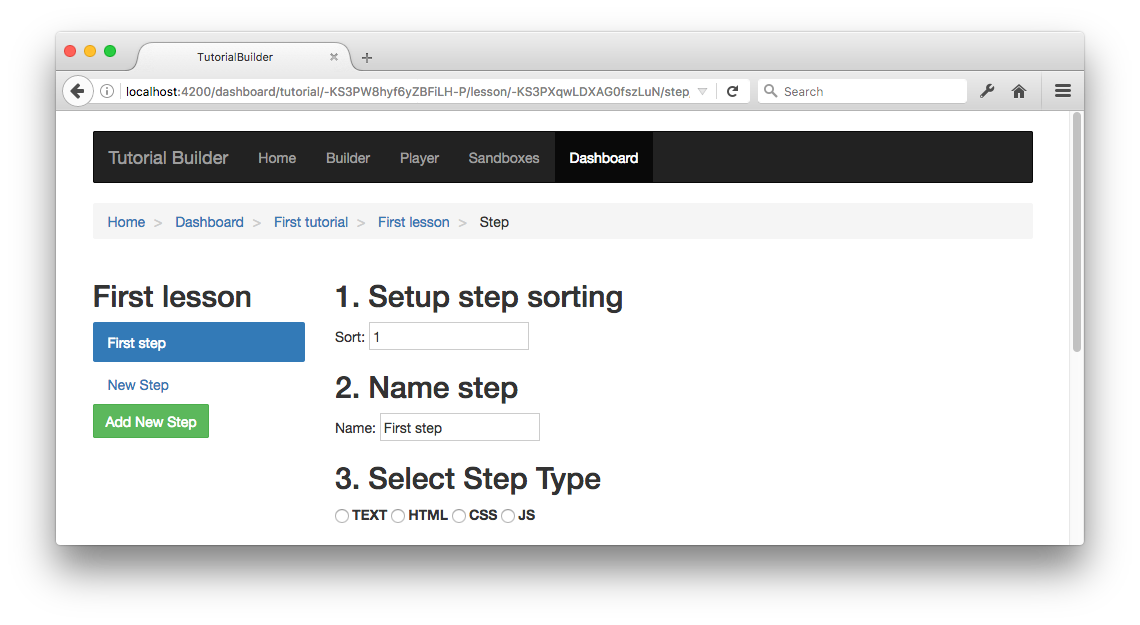
\includegraphics[width=1\textwidth]{assets/breadcrumb-screenshot.png}
\caption{Screenshot about breadcrumbs implementation}
\label{fig:breadcrumb-screenshot}
\end{figure}

\subsection{Communication between two components}

There is an interesting problem domain on JavaScript applications. When we build a JavaScript based single page application, we use little elements to build a larger section. These little elements are called components. Putting these components next to each other creates a webpage. Components are reusable, we have to create, develop them only once and we can insert them in different pages. The above explained breadcrumb is a component also, which was created by other developers, so we can just simply insert in our app.

However, these components do what they has to do independently and they do not worry too much about other part of the application. Except if we connect them together.

There is an other challenge in terms of components. What if we would like to insert a little part of a complex component to somewhere else in our application. For instance, we have a component which shows some data and we can paginate the data with buttons, but these buttons are somewhere else on the website and not directly around the data. Logically, we have to split the highly coupled component.

Luckily other developers already solved this problem. "Ember-wormhole" addon is added to the project, because this helps to insert functionally connected html elements on different part of the page.

In my step editor, there is an "Undo/Redo" button component, which belongs to the Step editor form. It is on the right side of the page. This wormhole plugin helped me to keep these two parts are connected.

You can see the implementation in Figure \ref{fig:wormhole}

\begin{figure}[ht]
\centering
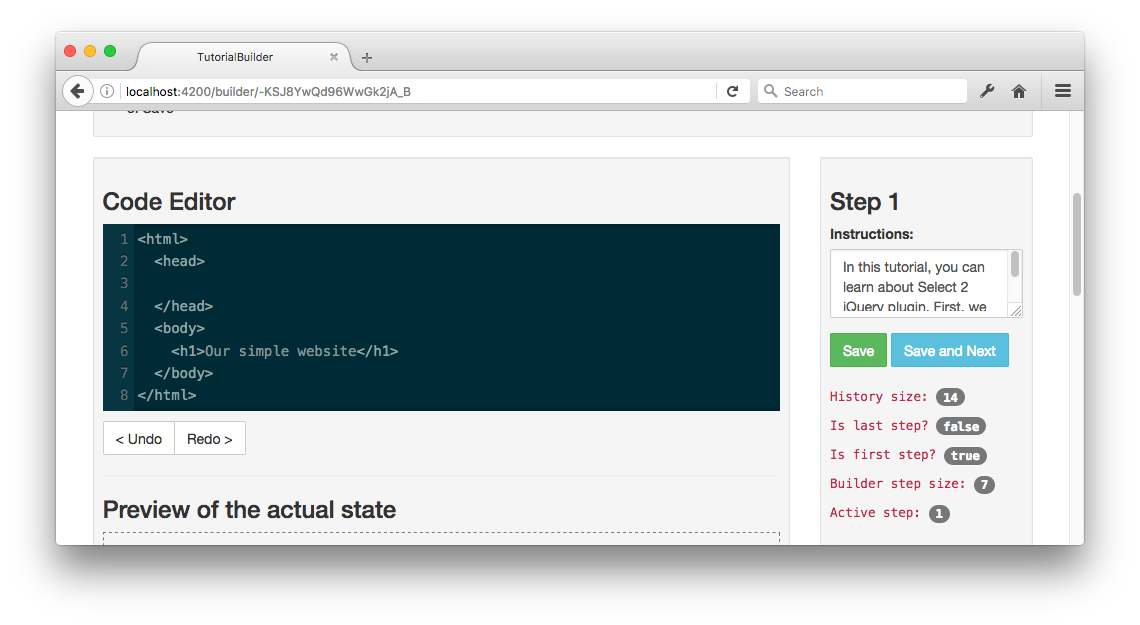
\includegraphics[width=1\textwidth]{assets/wormhole-screenshot.png}
\caption{Using Ember Wormhole}
\label{fig:wormhole}
\end{figure}

\subsection{Implemented database model} \label{database-implementation}

The demo app uses a nested model structure in the "Dashboard" section, which was suggested in the Design section (\ref{database-design}). During the implementation process, my first iteration tried to cover this wider use case (requirements R1, R2, R3, R7, R8), however, I realized, the challenge is not really on this area.

Finally I created a "builder" model and a "builder-step" model. (Requirements R13, R14.)

Builder model fields: name (string), builderSteps (hasMany)

BuilderStep model fields: builder (belongsTo), sort (number), comment (string), code (string)

With this simplified structure I was able to focus only the implementation of the tutorial and step builder functionality.

Figure \ref{fig:database-tables} summarizes these database tables and models.

\begin{figure}[htbp]
\centering
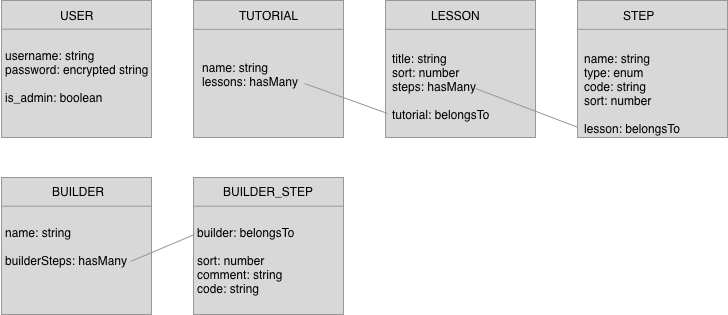
\includegraphics[width=1\textwidth]{assets/database-tables}
\caption{Database tables}
\label{fig:database-tables}
\end{figure}

The communication between the frontend and backend services is managed by adapters. The main adapter is the Firebase adapter which automatically updates data to the Firebase server. Firebase is a real time database. The limited, free to use version is enough for experimenting and for demo purposes.

The secondary adapter is a JSONApi Adapter. JSONApi \cite{jsonapi} is a new standard of data communication format which is the Ember.js default adapter. It is only active when I use Ruby on Rails based backend system. JSONAPi adapter is commented out in the production version, because I have not added all model to the Ruby on Rails app. I keep it there, because the further development of this project will focus on this backend instead of using Firebase.

\section{Challenges}

\subsection{Adding Emmet to Code Mirror} \label{emmet}

Emmet is an essential toolkit for web-developers, which can be added to most of the popular code editors. We can write html and css code using simple abbreviations only \cite{emmet}.

As I mentioned earlier, using Ember install, helped me to add the Code Mirror code editor. Unfortunately, this addon focuses only the very basic user scenarios, mainly for simple code editing.

Digging deep in the Ember Addon implementation, called Ivy-CodeMirror \cite{ivy-codemirror}, I found out how the Code Mirror instance is managed by this addon.

In my codebase, you can find a unique special component, which initialize Emmet with CodeMirror, when a code window added to the page. (Location of the component file: "app/components/ivy-codemirror.js")

Thanks to this changes, in my final implementation you can use this Emmet editing feature in each editor window. (Requirement R4.)

\subsection{Data stores}

Managing database and choosing the right solution always require more research and multiple iterations.

My project finally uses Firebase, as I planned in my proposal, however I had to try other options too. During the development process, I had problem with the speed of Firebase.

Firebase is a cloud based database, so it needs internet connection all the time. We cannot use the app offline. Additionally Firebase has limitations also.

Firstly, I tried to build a unique backend system in Ruby on Rails. You can find the actual state of this application on my Github \cite{tutorial-builder-backend}. I implemented a special saving mechanism in the code editor. When we modify the code in the editor, changes will be saved every third second automatically. Saving changes does not overheat the database.

However, implementing a full backend system is a big overhead in a smaller prototype project like this.

Secondly, I tried to use a mocking system, which is popular in Ember.js ecosystem. This mocking addon is called Ember Mirage \cite{ember-mirage}. When you use a mocking system in a frontend application, you can run the application without any backend support, because all the database related backend response is generated by an other JavaScript code. You can read and save data. It is super fast and easy to experiment with it. The only disadvantage of it is that the data is saved temporarily. If you close the web browser, all data will be deleted. Usually we use "fixtures" for pre populate the database when we open the app. I experimented with this mocking system, but finally I went back to Firebase, because it was important to me to upload the app to a public server, and to connect it to a real database. I have just continued the development process with Firebase.

\section{Reflection}

\subsection{Great part}

I think, it was great working on the architecture of this project. Thinking about the different elements and technology, and how these parts connect together. Working with Ember.js is fun and I learned a lot about this modern, matured frontend framework.

Building the backend system and trying different approaches were interesting, especially using Ruby on Rails, which is one of my favourite technologies.

I am impressed, how complex and advanced most of the web based code editor tools. Reviewing them gave me the opportunity to understand more, how they work. Adding Code Mirror to my project was a good choice, because it is feature heavy with an extensive public programming API.

\subsection {Need improvement}

As I already explained it in the challenging section, managing history, deleting or moving steps in a tutorial can be improved. I think, this is a great area for further project. The question is how can we maintain the consistency between steps, when we remove or move steps around. It is not only a technical challenge, it is more likely a UX problem.

\subsection {Would do differently?}

This project is about experimenting and learning new tools, solving problems and developing solutions. This process is obviously involve steps which does not produce real value at the end, however these steps are the necessary cost for finding the right direction.

I feel, my plan was too ambitious, and I had to realize that implementing what I imagined had its own challenges. Reducing the scope as early as possible is always better.

\chapter{Evaluation}

\section{Process}

The product evaluation has two parts. The first part is expert evaluation, which means, I collected feedbacks from my direct colleagues (from my workplace and from research group). In this section I describe the implemented product with screenshots. The second part is a survey, which helped to collect opinion about programming tutorial usage.

\subsection{Expert evaluation}

Expert evaluation helps to discover quickly the "low-hanging fruits", obvious usability problems without investing extra resource to organize a wider user testing session.

My research product is a prototype, which cannot be perfect for the first iteration, but it can already help us to direct our future study.

Expert evaluators were my colleagues. 4 developers and 1 UX designer. In each case I followed the same process. I showed them my prototype and I asked them to build a simple tutorial. The task was to create a tutorial with 3-4 steps which shows how to build a basic Hello World website with Bootstrap. I made notes of their feedback, questions and difficulties.

This evaluation focused on the content creator features, so the evaluators are represented our primary persona, the open source project maintainer or teacher persona.

Here is a walkthrough on how the app works, what it does containing feedbacks from the evaluators.

\newpage

\textbf{The home page}

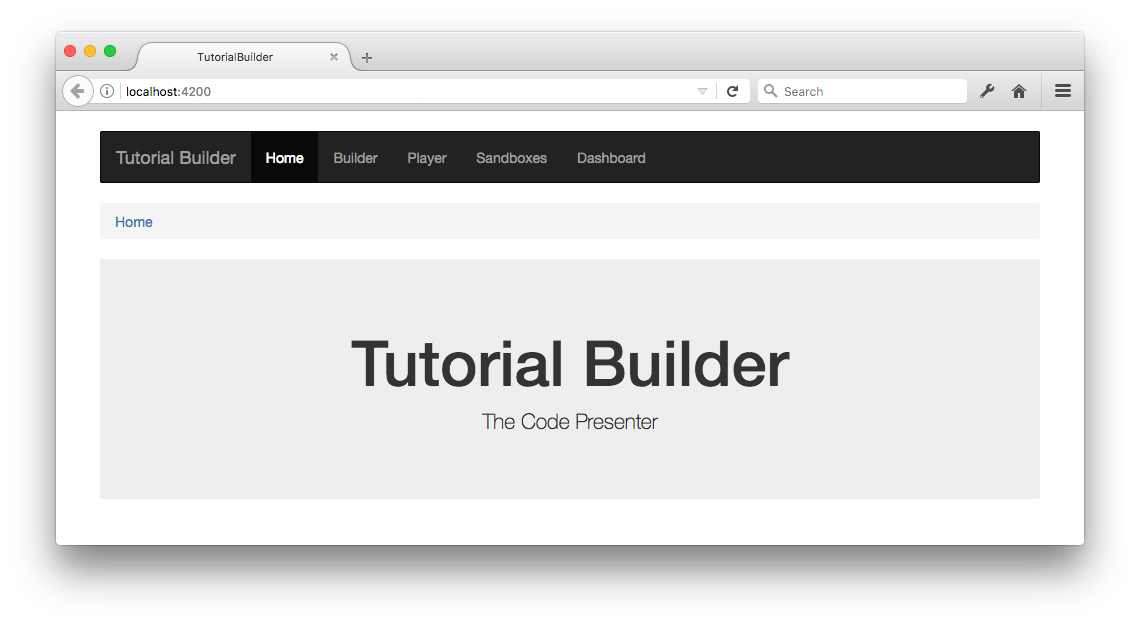
\includegraphics[width=1\textwidth]{assets/tour-screenshots/home-page.png}\\*[8pt]

Based on the feedbacks from the expert evaluators, there is a home screen with the title which serves mainly as a placeholder at the moment. Originally, there was not any homepage, but all evaluators mentioned the lack of it.

\newpage

\textbf{The Builder}

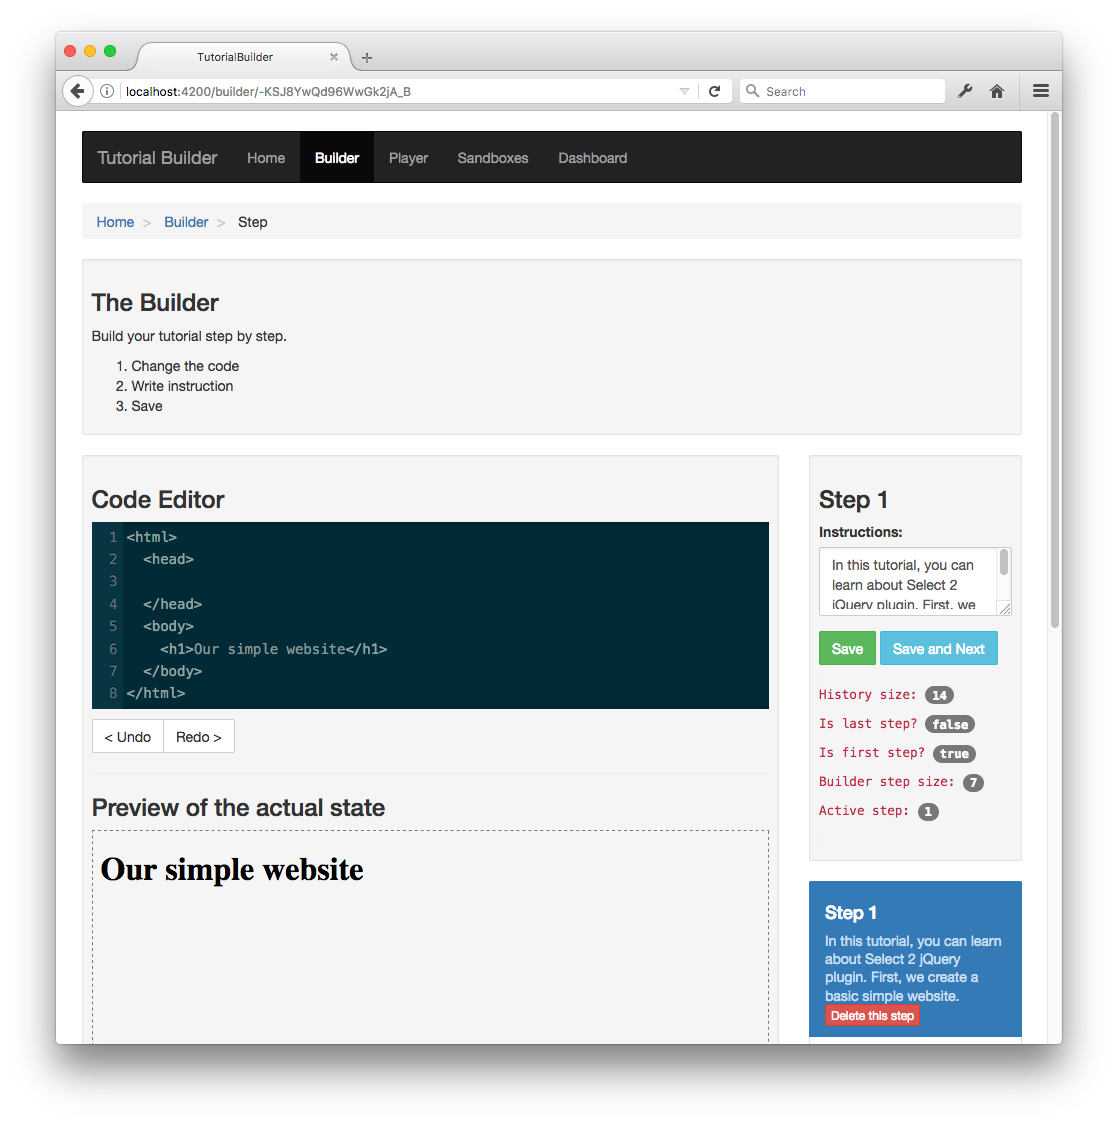
\includegraphics[width=1\textwidth]{assets/tour-screenshots/the-builder.png}\\*[8pt]

This screen is for the content creators, the admin area. The code editor is in the center, where the content creator can edit the source code and a step. On the right side, there is an instruction box. We can see the preview of the website. During the editing process, the application saves the history of changes, so the user can revoke or add new content. (Requirements R3-R6, R13.)

Reviewing this area with evaluators, one of the most important feedbacks was, how we can modify, drag and drop, delete steps; and how we can keep the consistency between steps. These feedbacks reflect the same questions we described in the Chapter \ref{history}. 4 out of 5 evaluators wanted to reorganize steps using drag and drop. 3 evaluators deleted steps and recognized the inconsistency between them  after this action. They manually adjusted the content in the connected steps in order to maintain consistency.

\newpage

\textbf{The Player}

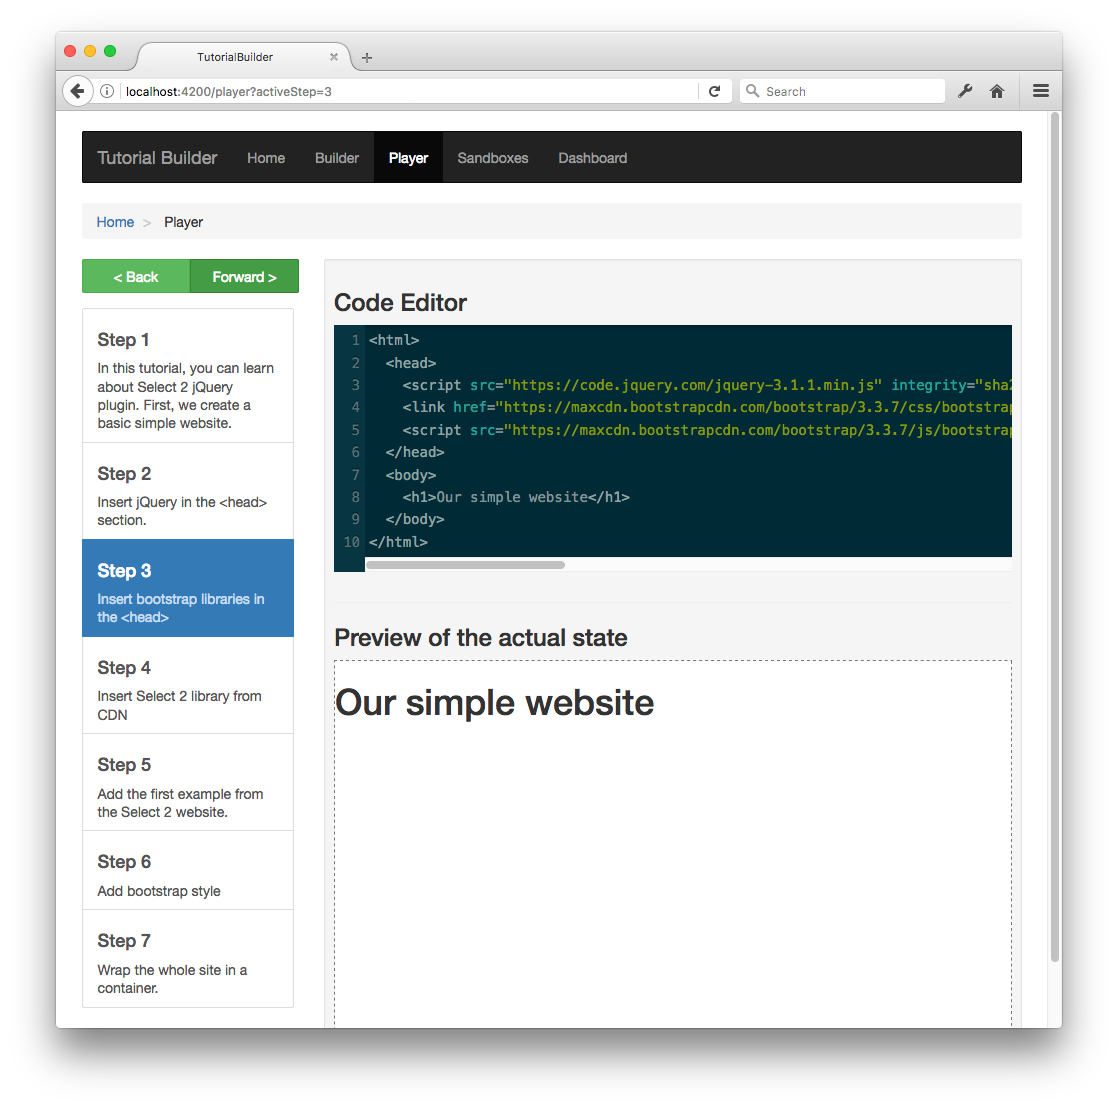
\includegraphics[width=1\textwidth]{assets/tour-screenshots/the-player.png}\\*[8pt]

This screen is for the content consumers, the player area. User can go forward and backward between steps. User can experiment with the code and can see the preview of the code example. (Requirements R8-R11.)

In the next chapter we read more about a survey which focuses of the secondary persona requirements.

\newpage

\textbf{Sandboxes}

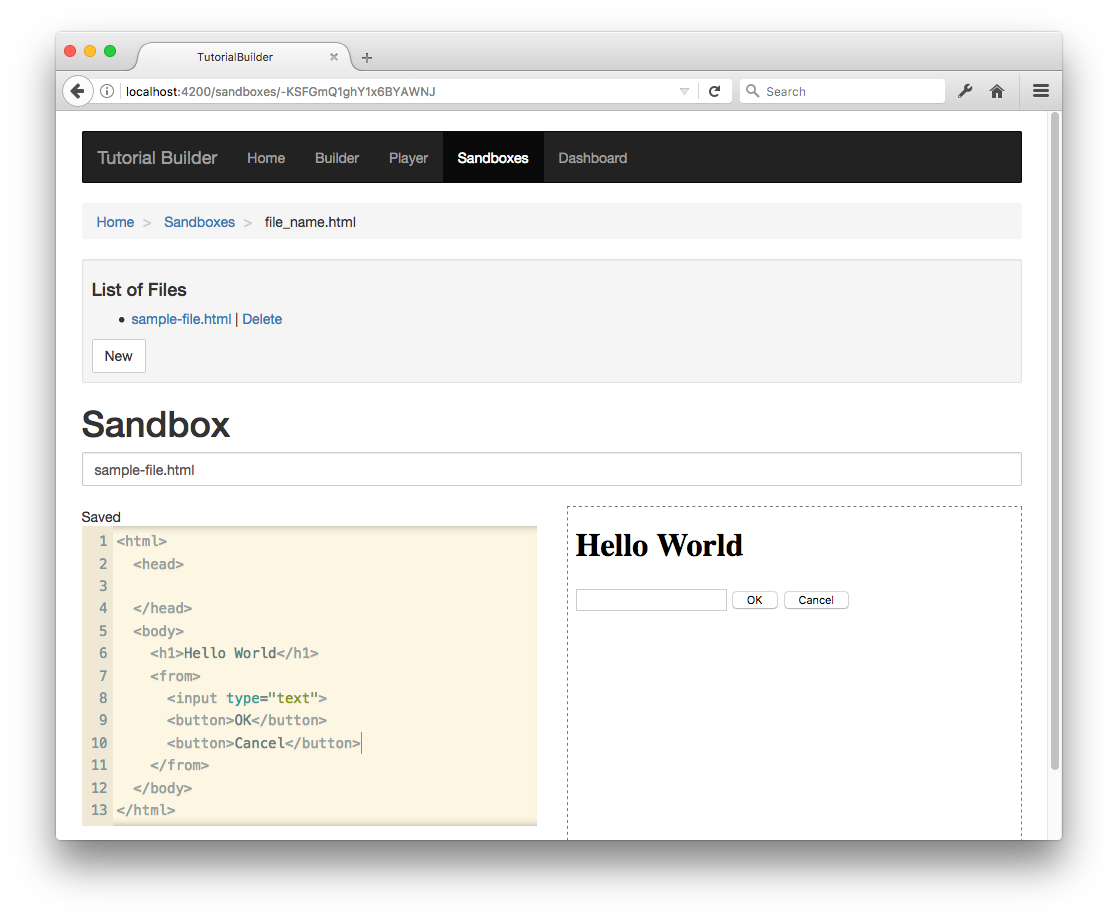
\includegraphics[width=1\textwidth]{assets/tour-screenshots/the-sandbox.png}\\*[8pt]

This part of the application was the first implementation of this prototype. It is a fully functional sandbox area where the user can create new files and can see realtime changes in the preview window. It is connected to the real time database. All changes are automatically saved. (Requirement R14.)

\newpage

\textbf{Dashboard}

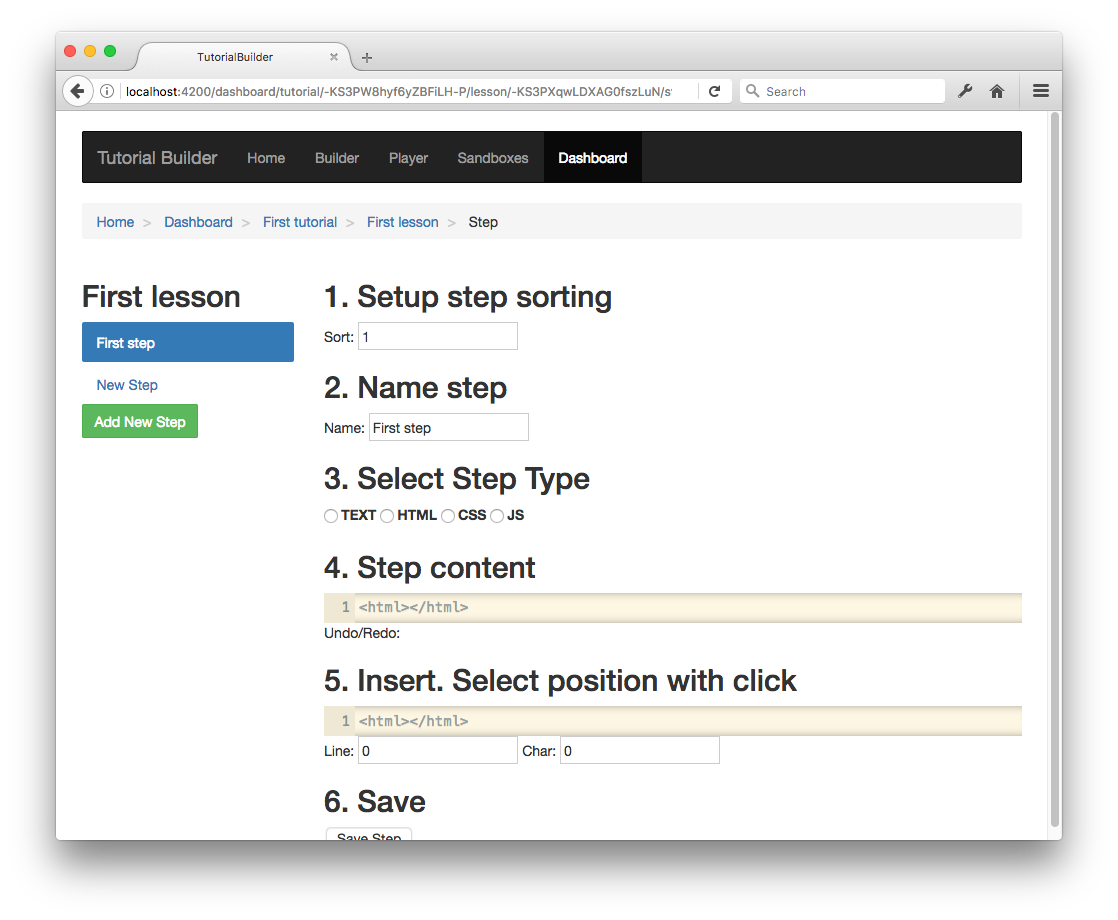
\includegraphics[width=1\textwidth]{assets/tour-screenshots/dashboard.png}\\*[8pt]

This area represents the described database model. In a realistic implementation we can create more tutorials, lessons, and steps. A step would have more types and it would behave differently based on the type of the content (text, html, css or js). (Requirements R1, R2, R7, R8.)

\newpage

\subsection{Tutorial Builder Survey}

Watching, reading or following tutorials are important part of our learning process, but everybody can have different motivation. I launched a survey for collecting information about user's motivation and their goals.

Victoria University ethics committee approved my request, so I was able to run a little campaign on my twitter, on my blog, and shared the link in different developer chat groups.

The survey focuses on our secondary persona. I tried to reach participants who more likely are tutorial content consumers, students, developers. For this reason, I shared the link on my tutorial website (\url{http://www.yoember.com}). This website's visitors are in our target group. I shared the link in Slack groups, mainly used by students and developers who would like to learn new skills. (Enspiral Dev Academy Slack Channel, Yoember Slack Channel, JavaScript New Zealand Slack Channel). Twitter was also efficient in the participant recruitment process as we can see in the Figure \ref{fig:twitter}

\begin{figure}[htbp]
\centering
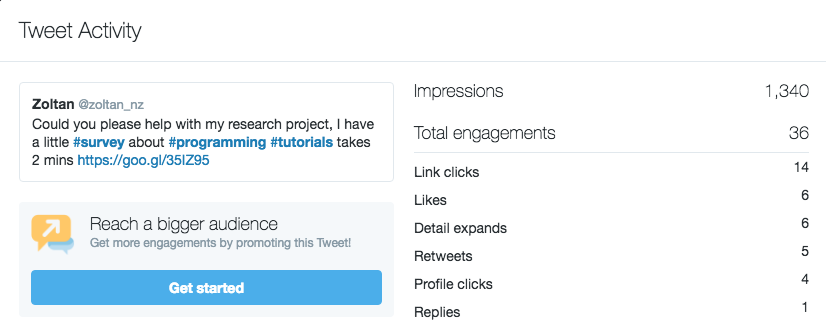
\includegraphics[width=1\textwidth]{assets/tweet-activity.png}
\caption{Tweet activity}
\label{fig:twitter}
\end{figure}

I built the survey on Google Survey platform, and it was presented as the following screenshot shows.

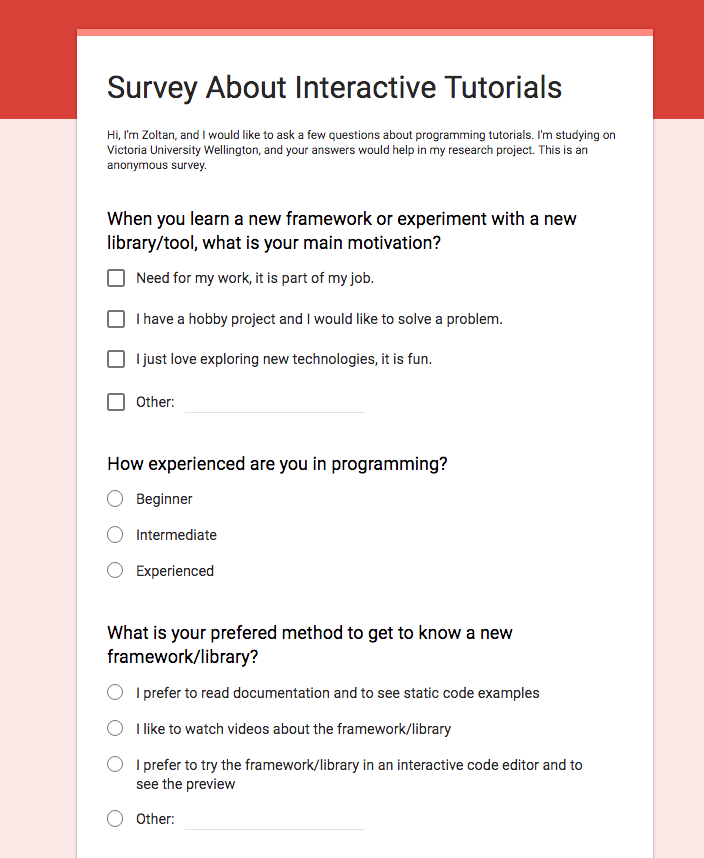
\includegraphics[width=1\textwidth]{assets/survey-screenshot.png}\\*[8pt]

\textbf{The questions and options:}

\noindent When you learn a new framework or experiment with a new library/tool, what is your main motivation?
\begin{itemize}[noitemsep]
\item Need for my work, it is part of my job
\item I have a hobby project and I would like to solve a problem.
\item I just love exploring new technologies, it is fun.
\item Other...
\end{itemize}

\noindent How experienced are you in programming?
\begin{itemize}[noitemsep]
\item Beginner
\item Intermediate
\item Experienced
\end{itemize}

\noindent What is your prefered method to get to know a new framework/library?
\begin{itemize}[noitemsep]
\item I prefer to read documentation and to see static code examples
\item I like to watch videos about the framework/library
\item I prefer to try the framework/library in an interactive code editor and to see the preview
\end{itemize}

\noindent When you try a library or a framework in a web based code editor, which features are important to you? (Scale from 1-not important to 6-very important)
\begin{itemize}[noitemsep]
\item There is a step by step introduction of the usage of the library
\item I can pause, reverse the introduction
\item I can modify the code in the web based code editor
\item I can share/export/copy the code from the web based code editor
\end{itemize}

What other features would you like to see in a web based interactive tutorial.
(open question)

\subsection{Survey analysis}

The survey was running for 3 weeks and I got 82 answers. Contributors are from 20 different countries. 49.35\% from New Zealand, 16.88\% from USA and 5.19\% from Canada. I also received answers from India, Australia, Hungary, Ireland, Brazil, Estonia, Germany, and a few other countries.

The Histogram of Age shows the distribution of ages. Ranges from 20 to 55. The median is 32.

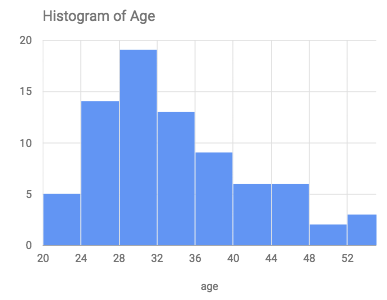
\includegraphics[width=1\textwidth]{assets/survey-result/histogram-of-age.png}\\*[8pt]

To the question about the main motivation for learning new library or tool more than 61\% answered that they just love exploring new technologies and for 43\% needs it for their job.

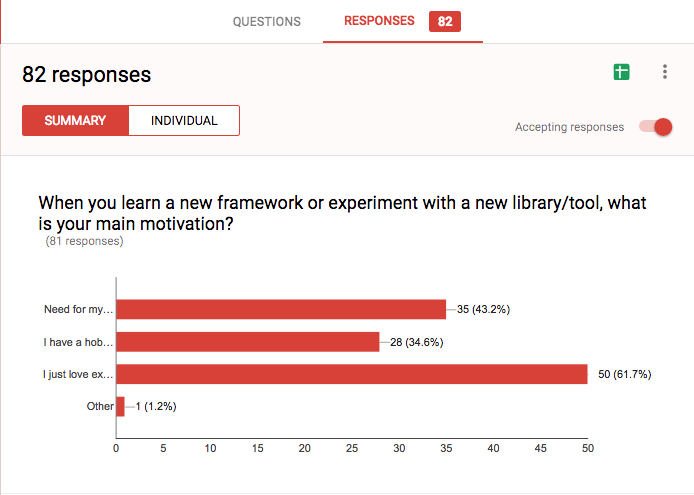
\includegraphics[width=1\textwidth]{assets/survey-result/main-motivation.png}\\*[8pt]

Only 14.8\% of the participants determined themselves as beginners, and almost half of the responders are experienced developers.

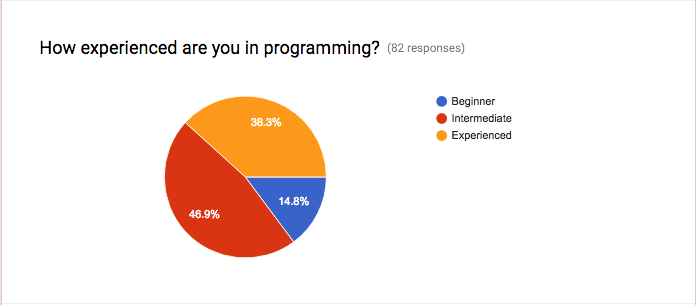
\includegraphics[width=1\textwidth]{assets/survey-result/how-experienced.png}\\*[8pt]

The majority of people prefers to read documentation and checks static code examples when they learn a new framework or library. 30.9\% answered that they like to watch videos about the tool and only 22.2\% try in an interactive code editor.

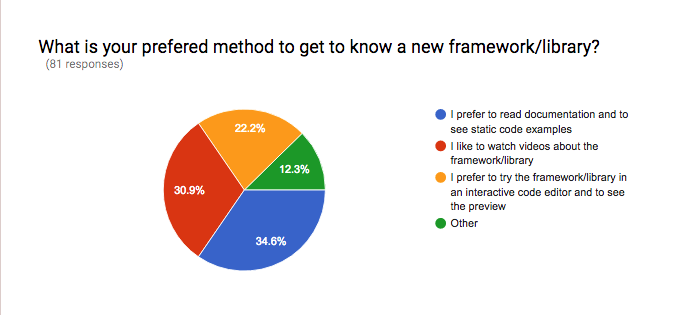
\includegraphics[width=1\textwidth]{assets/survey-result/prefered-method.png}\\*[8pt]

It is interesting to see which features are important in a tutorial. As we can read in the following graphs that the majority of responders would prefer these features:
\begin{itemize}[noitemsep]
\item step by step introduction of the usage of the library
\item can pause, reverse the introduction
\item can modify the code in a web based code editor
\end{itemize}

The "share, export or copy" feature is less important.

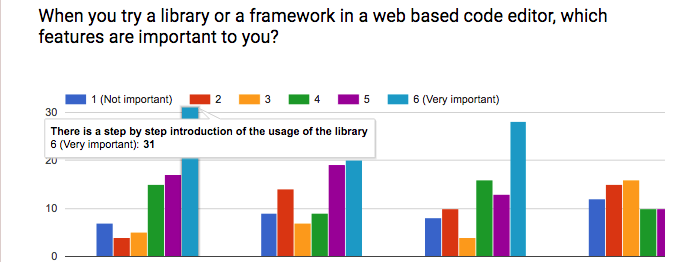
\includegraphics[width=1\textwidth]{assets/survey-result/features-stepbystep.png}\\*[8pt]

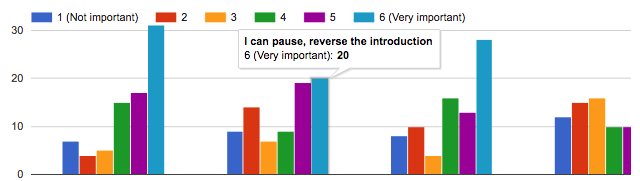
\includegraphics[width=1\textwidth]{assets/survey-result/features-paused.png}\\*[8pt]

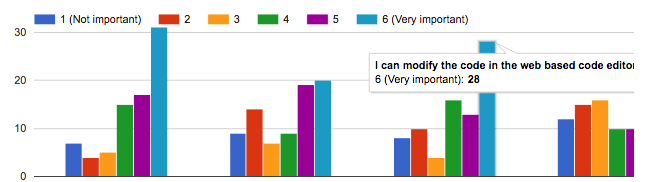
\includegraphics[width=1\textwidth]{assets/survey-result/features-modify-code.png}\\*[8pt]

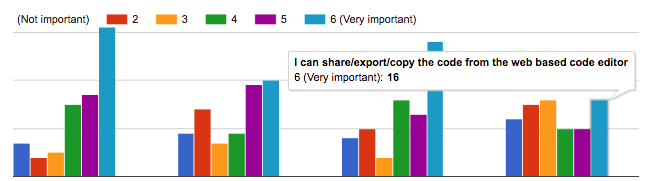
\includegraphics[width=1\textwidth]{assets/survey-result/features-sharing.png}\\*[8pt]

The survey shows that the developers still prefer reading a good documentation when they experiment with a new library or framework, however if there would be some interactive option they would play with this dynamic introduction.

The survey helps to determine the focus of the most important features in future work. The interactive code editor, and the function of forward/backward playing of the steps is important, however sharing, copying code are less important.

\chapter{Summary}

\section{Conclusion}

Working on a project like this helped me to experiment with solutions, and I learned a lot how I can connect together different parts of a complex problem.

We built an online publishing prototype where we use code editor and step by step instructions to present programming challenges and solutions in order to solve a computer science problem.

The prototype has two parts, an administration area, a builder, where the content creator can build a tutorial, and a player tool, where the recorded steps are presented.

Additionally, we have a sandbox area in this application, where we can practice website building.

The fourth section of the application is a complex dashboard, which presents a more realistic structure of a possible tutorial builder.

During the project there were technical and user experience challenges. For instance, the frontend development was separated from the backend development, and it provided flexibility, however it caused problem with scalability, especially when the backend system is a remote cloud based datastore. Using online code editor in a web browser is a special area. From one hand, it is a technical challenge to add an editor to a website, form the other hand, it has to be user friendly and easy to use.It should provide almost the same experience as a desktop software developer editor. It was also interesting  to deal with different types of information (text, code, history log), and structure the data and save them  in a database.

After describing the problem, the requirement list was ambitious, but it was almost fully implemented. The content creator, for example a teacher, can navigate to an Admin page (R1), can create a new tutorial (R2), can add steps (R3) and different content (R4), can modify these steps  (R5). A content consumer can see a list of tutorials (R7), can see the steps (R8) in order (R9), can navigate among them (R10, R11). The implementation shows different user interfaces (R12). There are two versions of layout, one for the content creator (R13) and one for the consumer (R14).

One of the requirements was that (R6), how all steps can stay in sync automatically after reorganizing them in a tutorial. This special problem was implemented partly. It has been discussed in details in Section \ref{history}, however it is a good candidate for future work.

\section{Future work}

The step by step tutorial is just the beginning. I already visualized a much bigger project which actually can be really helpful for teachers and for students also.

My original plan was to show how you can build a more complex application. When we build a web app, we deal with a bunch of files and complex directory structure. So many moving parts. Keeping this in sync and showing the changes of directories and file content, we usually use git in software development. One of the obvious choices would be to bring together a step-by-step builder tool, like this prototype, and git repository management. Each git commit would be a step in the tutorial. Most of the git repository management websites has a public API. Git repository API can help us to show the steps on our website, in our code editor. However it would introduce the same problem that we already encountered in this prototype. How can we go back in time and change to an earlier step while keeping the history and consistency? The answer lies in Human Computer Interaction, in UX.


%%%%%%%%%%%%%%%%%%%%%%%%%%%%%%%%%%%%%%%%%%%%%%%%%%%%%%%

\backmatter

%%%%%%%%%%%%%%%%%%%%%%%%%%%%%%%%%%%%%%%%%%%%%%%%%%%%%%%

\bibliographystyle{acm}

\begin{thebibliography}{9}

\bibitem{cm-movie}
CodeMirror Movie - \url{https://github.com/sergeche/codemirror-movie}

\bibitem{tiobe}
Tiobe.com - \url{http://www.tiobe.com/tiobe_index}

\bibitem{firebase}
Firebase - \url{https://firebase.google.com}

\bibitem{jsonapi}
JSON Api - \url{http://jsonapi.org}

\bibitem{surge}
Surge.sh Static Website Hosting Service - \url{http://surge.sh}

\bibitem{clean-code}
Book: Robert C. Martin - Clean Code - ISBN-13: 978-0132350884

\bibitem{es6}
ES6 Standard - \url{http://www.ecma-international.org/ecma-262/6.0/}

\bibitem{solid}
SOLID pattern - \url{https://en.wikipedia.org/wiki/SOLID_(object-oriented_design)}

\bibitem{bootstrap}
Bootstrap - \url{http://getbootstrap.com}

\bibitem{less}
Less - \url{http://lesscss.org/}

\bibitem{sass}
Sass - \url{http://sass-lang.com/}

\bibitem{emmet}
Emmet - \url{http://emmet.io/}

\bibitem{ivy-codemirror}
Ivy-CodeMirror - \url{https://github.com/IvyApp/ivy-codemirror}

\bibitem{ember-crumbly}
Ember-Crumbly Addon - \url{https://github.com/poteto/ember-crumbly}

\bibitem{tutorial-builder-backend}
Tutorial Builder Backend - Ruby on Rails app \url{https://github.com/zoltan-nz/tutorial-builder-backend}

\bibitem{ember-mirage}
Ember Mirage - \url{http://www.ember-cli-mirage.com/}

\end{thebibliography}

%%%%%%%%%%%%%%%%%%%%%%%%%%%%%%%%%%%%%%%%%%%%%%%%%%%%%%%

\end{document}
